\documentclass{beamer}
\usepackage[utf8]{inputenc}
\usepackage{multimedia}
\usepackage[final]{pdfpages}
\usetheme{Dresden}%Goettingen}%Warsaw}
\usecolortheme{lily}
\setbeamertemplate{footline}[page number]
\title[Fast classification]{Efficient dynamic and static environment classification in Occupancy Grid framework}
\author{Jander Nascimento}
\institute{Université Joseph Fourier / INRIA}
\date{\today}
\begin{document}

\begin{frame}
\titlepage
\end{frame}

%\AtBeginSubsection[]
{
  \begin{frame}<beamer>
    \frametitle{Roadmap}
    \tableofcontents%[currentsection,currentsubsection]
  \end{frame}
}

	\section{Introduction}
	
	\begin{frame}
		\frametitle{ADAS/ITS}
		
		\begin{columns}[t]
		  \begin{column}{5cm}
			\begin{exampleblock}{Stands for}	
				Advanced Driver Assistance Systems, cope with vehicle handling tasks
				
				Intelligent Transportation Systems
			\end{exampleblock}		
			\begin{block}{Goal}
				\begin{itemize}
				\item Reduce the risk of collisions
				\item Reduce the driver overload
				\item Increase the confort
				\end{itemize}
			\end{block}
		  \end{column}
		  
		  \begin{column}{5cm}
		  \begin{figure}[h]
			\center
			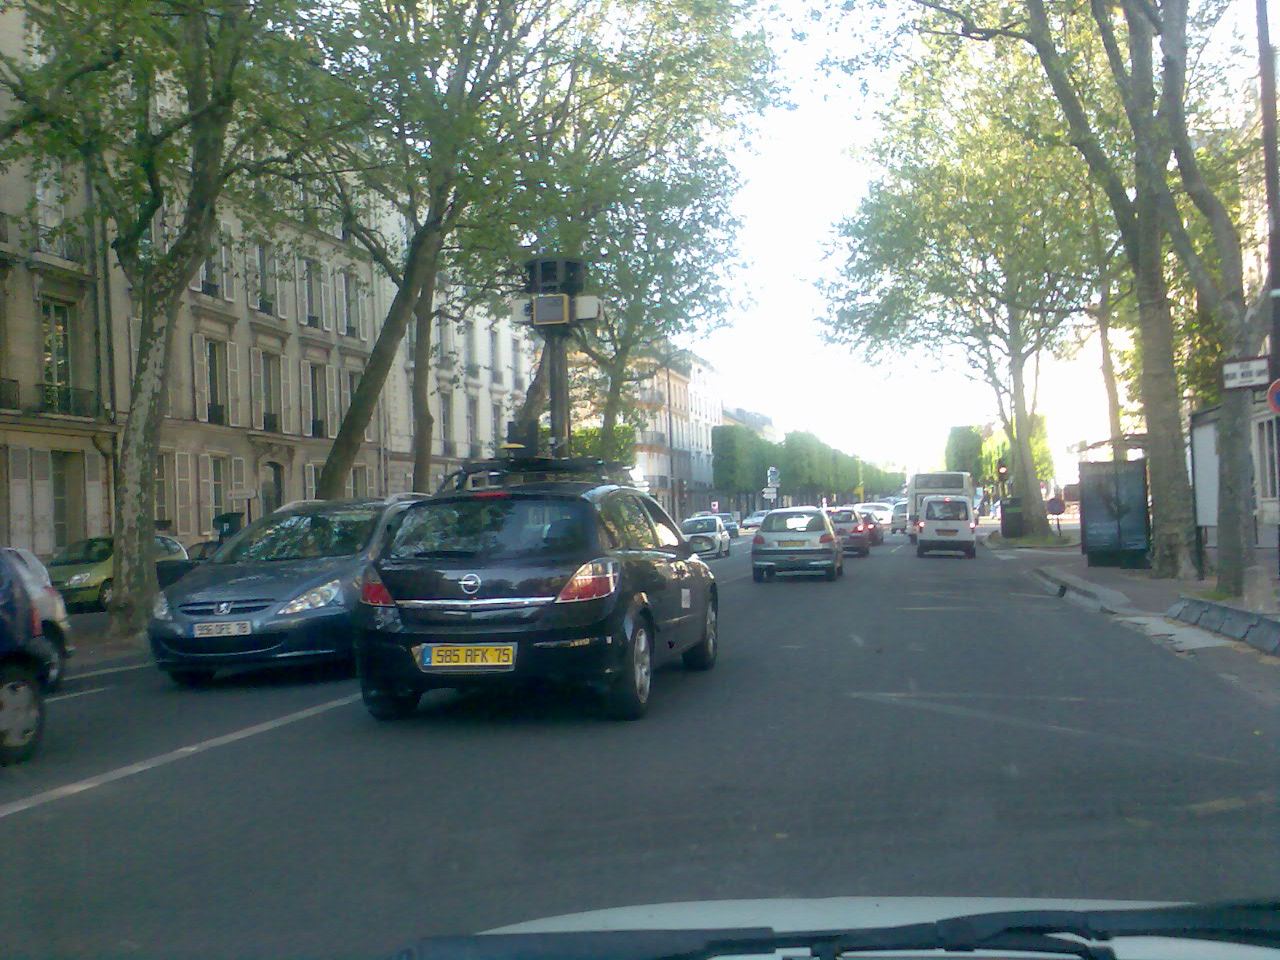
\includegraphics[scale=0.15]{img/fig:street:urban}
		  \end{figure}   
		  \end{column}
		 \end{columns}

	\end{frame}	

	\begin{frame}
		\frametitle{ADAS application architecture}	
		
		\begin{columns}[t]
		  \begin{column}{6cm}

			\begin{block}{Sensors}
					The means of perceiving the environment based on physical properties (cameras, lasers, etc.)
			\end{block}		

			\begin{block}{Perception}
					The process of acquiring knowledge about the environment \cite{iyengar1991autonomous}
			\end{block}		

			\begin{block}{Risk estimation}
					Evaluate the state space and assess the safety of the movement
			\end{block}				  

		  
		  \end{column}
		  
		  \begin{column}{6cm}
			\begin{figure}[h]
				\center
				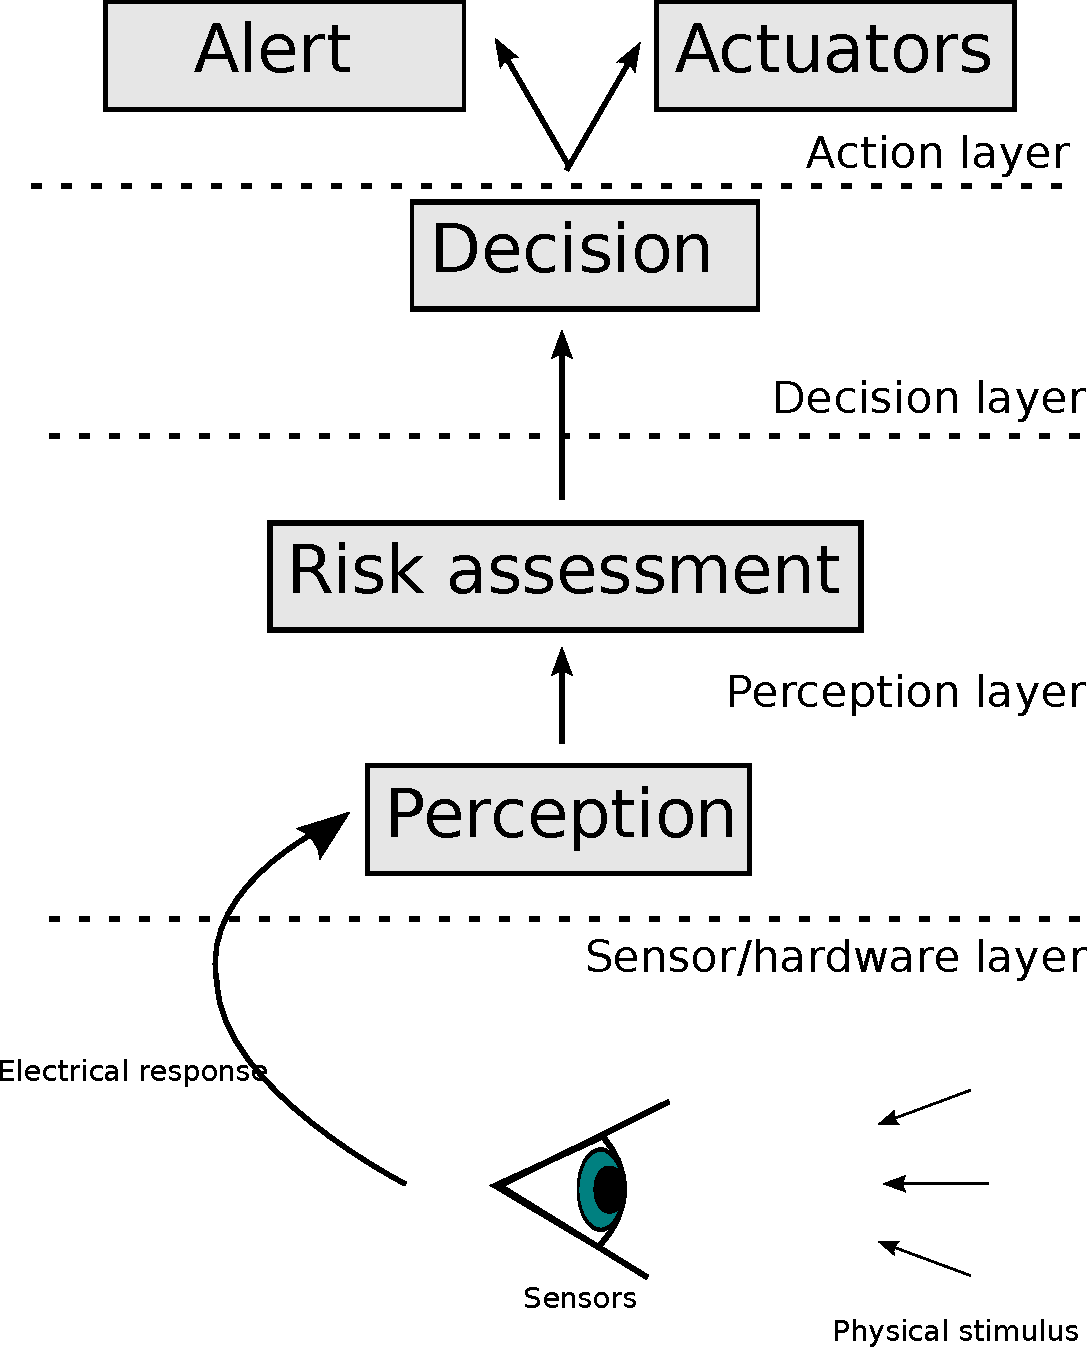
\includegraphics[scale=0.23]{../img/fig:sensors:roles}
			\end{figure}
		  \end{column}
		 \end{columns}		
		

		
		%\begin{exampleblock}{SLAM}		
		%	\begin{quotation}
%... providing the vehicle with a map of static parts of the environment as well as its location in the map %\cite{DBLP:journals/inffus/VuBA11}
%			\end{quotation}
%		\end{exampleblock}					
				
%		\begin{exampleblock}{DATMO}		
%			\begin{quotation}
%			... being aware of dynamic entities around, tracking them, and knowing their future position \cite{DBLP:journals/inffus/VuBA11}
%			\end{quotation}				
%		\end{exampleblock}						
				
	\end{frame}
	
	\begin{frame}
		\frametitle{Problem statement - BOF overview}
	
		  \begin{columns}[t]
		  \begin{column}{5cm}
			\begin{figure}[h]
			\center
	
		\begin{block}{Stands for..}
			Bayesian Occupancy Filter
			
			A perception framework developed in E-Motion team.  (ref)
		\end{block}
	
			\begin{block}{Short definition}
			\begin{itemize}		
				 \item Grid based representation of the environment
				 \item For each cell it calculates 2 probabilities:
			 		\begin{itemize}		
				 		\item probability of \textbf{occupancy} of the cell
				 		\item probability of \textbf{velocity} of cell
	 				\end{itemize}		
				 
			\end{itemize}				
			\end{block}
		\end{figure}	
		  \end{column}
		  
		  \begin{column}{5cm}
			\begin{figure}[h]
			\center
			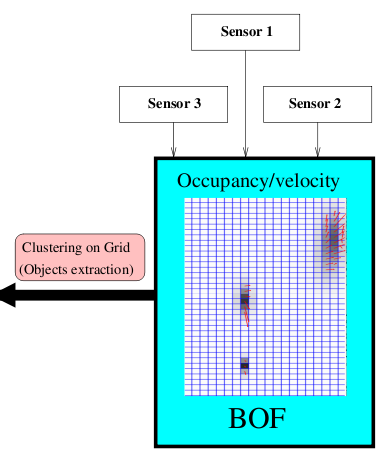
\includegraphics[scale=0.3]{img/bof}
		\end{figure}	
		  \end{column}
		 \end{columns}		
		
		
		
	\end{frame}

	\begin{frame}
		\frametitle{Context - Problem statement}

		BOF calculates velocities as Bayesian inference without using motion sensors
		
		\begin{itemize}
		\item Uses pre-defined range of velocities
		\item Needs to use the neighborhood for calculate those velocities
		\end{itemize}

		 \begin{alertblock}{Issue}
		 Needs to evaluate velocity distribution even for cells belonging to static parts
		 \end{alertblock}

		
	
		\begin{block}{Problem statement}		
			How to separate the input data from the laser into dynamic and static parts using information from the motion sensors?
			
			That can be used for BOF to concentrate its calculations for cells belonging to dynamic parts only.
		\end{block}
		
	\end{frame}

	\begin{frame}
		\frametitle{Perception}
	
			\begin{block}{Definition}
				the process of getting information from the environment using sensors
			\end{block}	
	
		  \begin{columns}[t]
		  \begin{column}{4cm}
		  	\small
			\begin{exampleblock}{SLAM}		
		
			\begin{itemize}
			\item Localization
			\item Mapping
			\end{itemize}			
			
			\end{exampleblock}					
				
		\begin{exampleblock}{DATMO}		
			\begin{itemize}
			\item Moving objects: Detection and Tracking
			\end{itemize}			
			
		\end{exampleblock}	
		  \end{column}
		  
		  \begin{column}{6cm}
			\begin{figure}[h]
			\center
			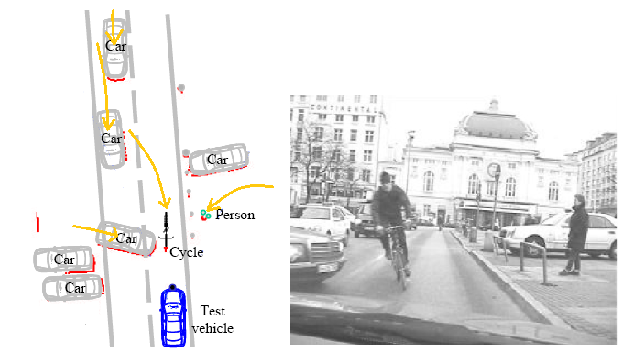
\includegraphics[scale=0.3]{img/perception}
		\end{figure}	
		  \end{column}
		 \end{columns}		 	
	
					
	
	\end{frame}	
	
%	\begin{frame}
%		\frametitle{Behavior-based risk estimation}
		
%		\begin{block}{Statistics}
%		75\% of the accidents are between two vehicles \cite{Hurt_1981}. Leaving only 25\% for all other causes.
%		\end{block}
%
%		\begin{exampleblock}{How tackle this issue?}
%		Behavior-base risk estimation (moving or static) is a feasible approach.
%		\end{exampleblock}
%
%		\begin{alertblock}{Idea}
%			Evaluate the risk based for the moving objects of the scene. Thus, leaving only moving objects in the binary grid.
%		\end{alertblock}
%
%		$<$image of a grid, with moving object extracted$>$

%	\end{frame}
%%%%%%%%%%%%%%%%%%%%%%%%%%%%%%
\section{State of the art}

	\begin{frame}
		\frametitle{State of the art}
		
		%\begin{block}{Other static/dynamic classification}
			\begin{itemize}
			\item Use a Single Camera for Simultaneous Localization And Mapping with  Mobile Object Tracking in dynamic environments \cite{Migliore_2009_ICRA}
				\begin{itemize}			
				\item Observe features at 3 different positions
				\item Needs feature association
				\item Not applicable for outdoors environment 
				%based on observerving same fereature from 3 diff positions, if the same feature is not in the same position detect as moving, problem feature association, only for indoors env. 
				\end{itemize}		
			%\item Mapping in dynamic environments using stereo vision \cite{DBLP:conf/ivs/LategahnGHKE11}
			%	\begin{itemize}
			%	\item Disparity image to find the contour
			%	\item Classifier based on SPRT				
			%	\end{itemize}		
			\item Grid-based localization and local mapping with moving object detection and tracking \cite{Vu201158}
				\begin{itemize}		
				\item Maximum likelihood based localization	
				\item Motion detection based on inconsistence between free and occupied space
				\item Solves the complete SLAM
				\end{itemize}	
			\end{itemize}		
		%\end{block}
	\end{frame}

%%%%%%%%%%%%%%%%%%%%%%%%%%%%%%

\section{Motion detection}

	\begin{frame}
		\frametitle{Solution overview}
		\begin{figure}[h]
			\center
			%\includegraphics[scale=0.5]{img/fig:problem}
			\includegraphics[scale=0.6]{img/fig:motion:overview:01}
		 \end{figure}
		 (replace clinder by the 2x sensor image)
		\begin{block}{Goal}
			 Being able to identify the dynamic parts of the environment
		\end{block}
		 
		\begin{block}{Result}
			Motion Grid, equivalent to input grid with high probability only for cells detected as moving
		\end{block}				 

		\begin{alertblock}{Not our goal}
			Solve SLAM
		\end{alertblock}
	\end{frame}

\subsection{preprocessing}

	\begin{frame}
		\frametitle{Experimental Platform}
		\begin{columns}[t]
		  \begin{column}{5cm}
		  \begin{figure}[h]
			\center
			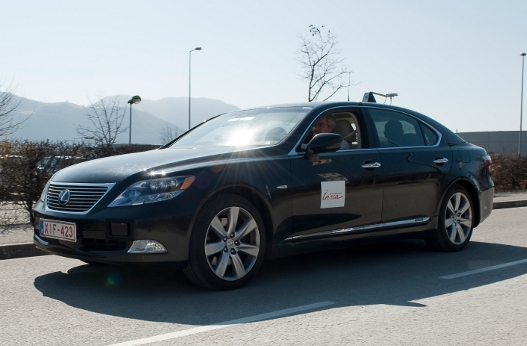
\includegraphics[scale=0.25]{../img/testbed:car}
		  \end{figure}	
		  \end{column}
		  
		  \begin{column}{5cm}
		  \begin{figure}[h]
			\center
			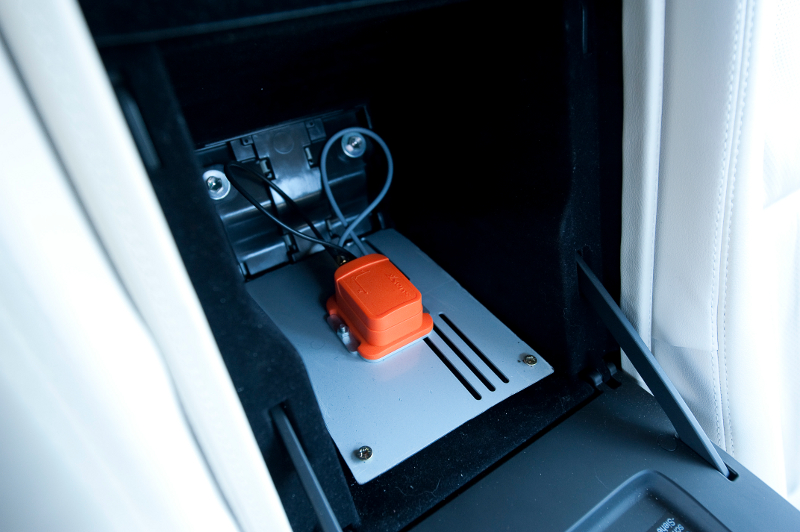
\includegraphics[scale=0.7]{../img/testbed:xsens}
		  \end{figure}   
		  \end{column}
		 \end{columns}			
		
		  \begin{columns}[t]
		  \begin{column}{5cm}
		  \begin{figure}[h]
			\center
			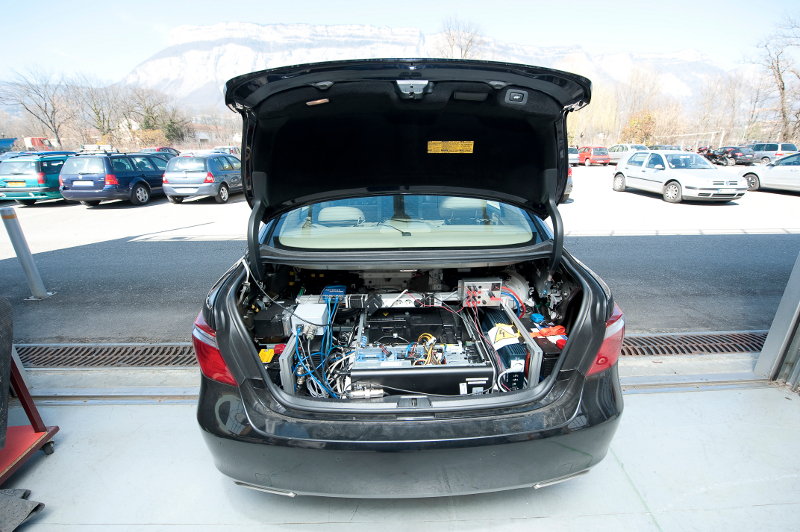
\includegraphics[scale=0.7]{../img/testbed:trunc}
		  \end{figure}
		  \end{column}
		  
		  \begin{column}{5cm}
		  \begin{figure}[h]
			\center
			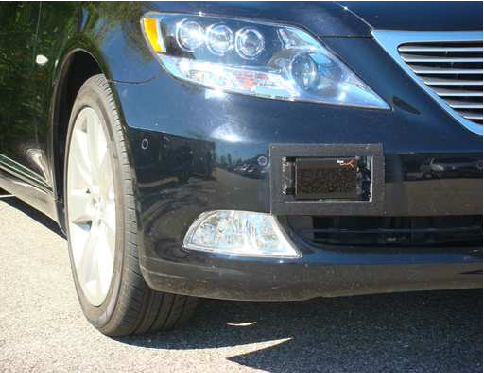
\includegraphics[scale=0.26]{../img/testbed:ibeo}
		  \end{figure}   
		  \end{column}
		 \end{columns}		 
	\end{frame}

	\begin{frame}
		\frametitle{Experimental Platform - laser configuration}	



		 \begin{columns}[t]
		  \begin{column}{5cm}

		  \begin{figure}[h]
			\center
			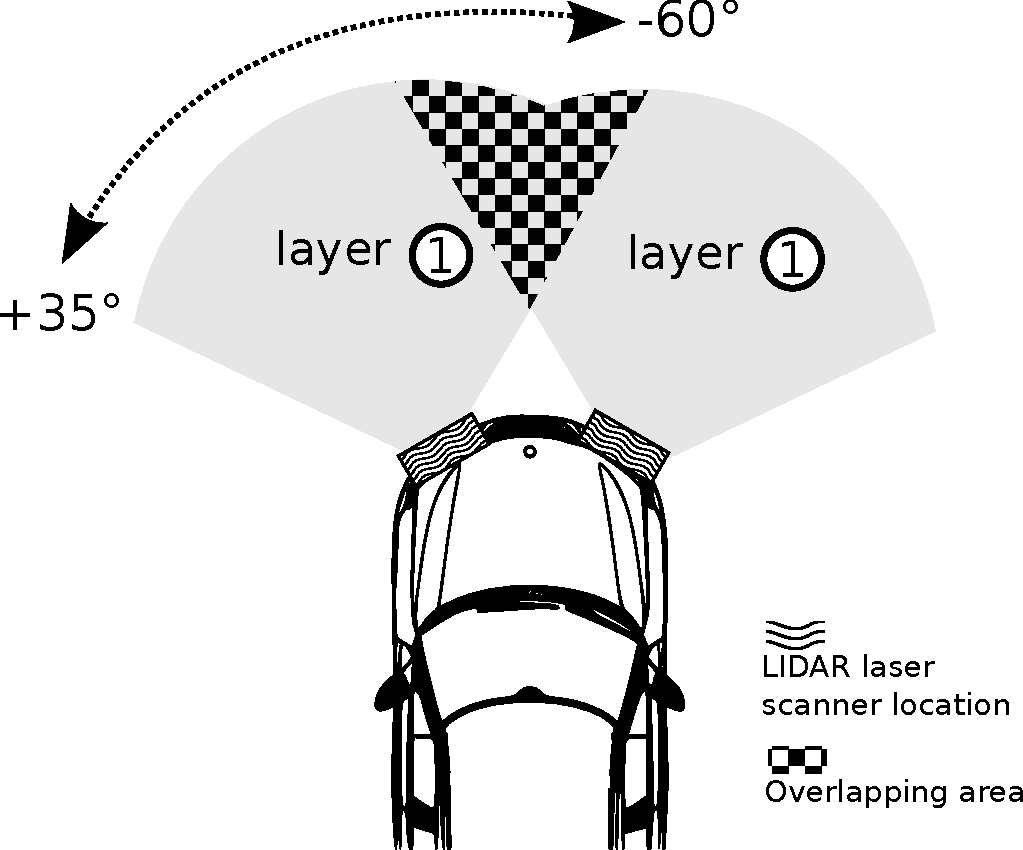
\includegraphics[scale=0.27]{../img/fig:demonstrator:superior:overlap}
		  \end{figure}   

		  \end{column}

		  \begin{column}{5cm}
		 \begin{figure}[h]
			\center
			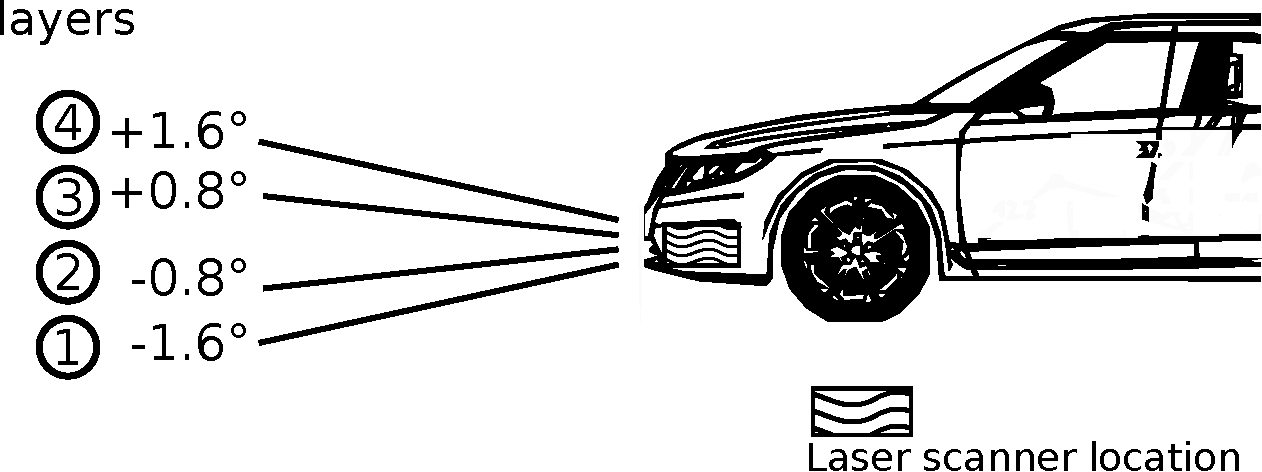
\includegraphics[scale=0.27]{../img/fig:demonstrator:lateral}
		\end{figure}		  
		  \end{column}
		 \end{columns} 	
	
	\end{frame}

	\begin{frame}
		\frametitle{Input preparation}
		\begin{figure}[h]
			\center
			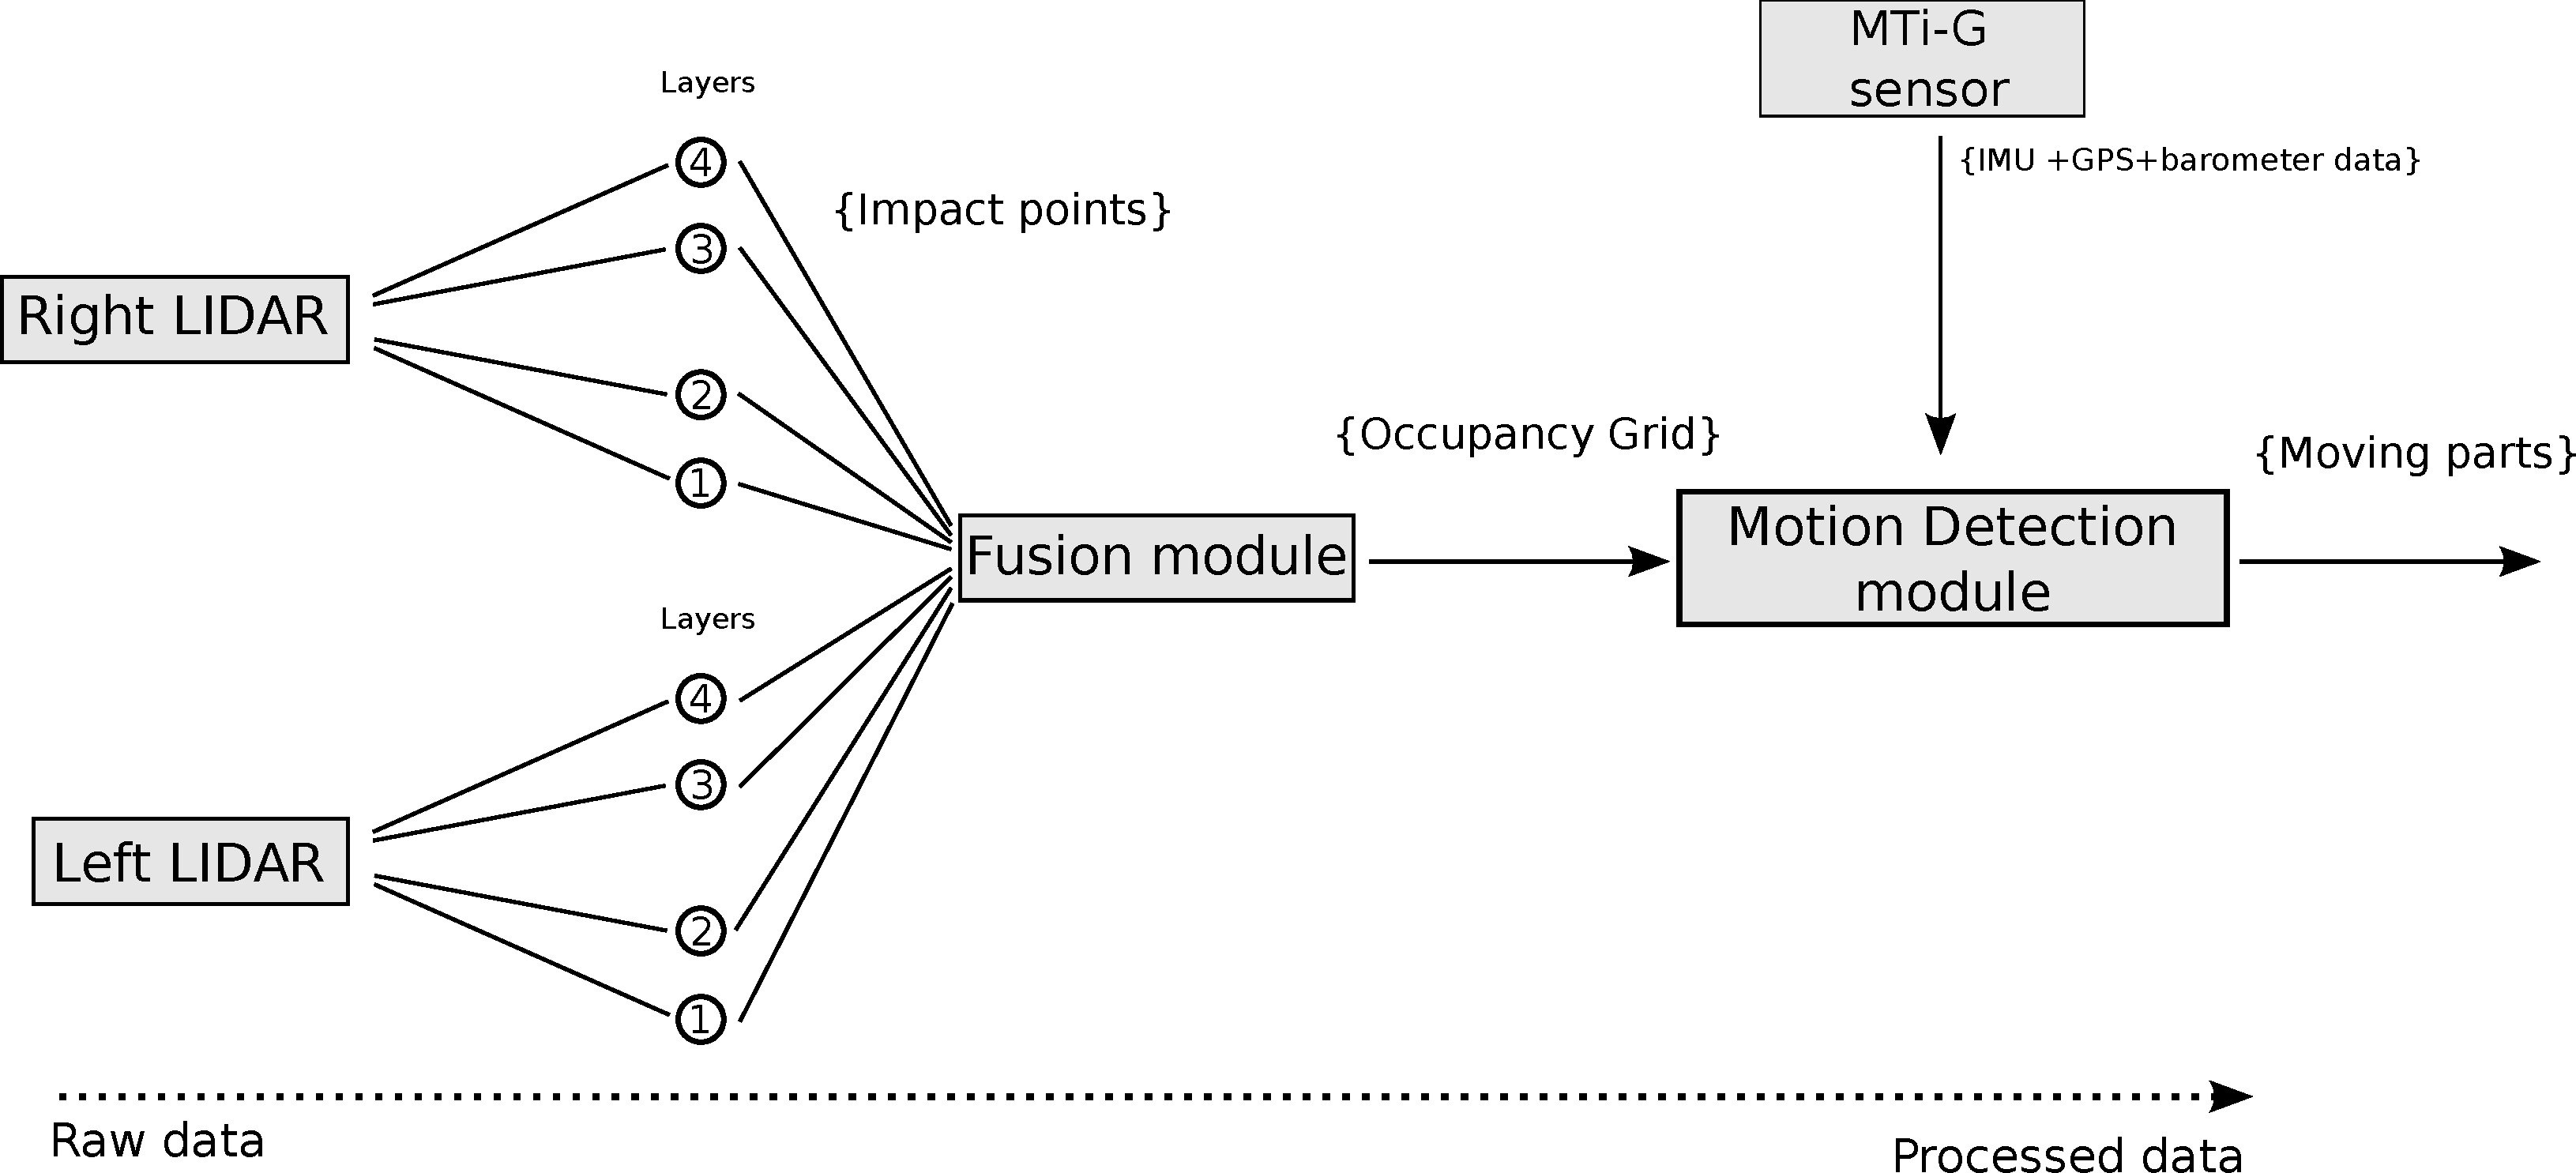
\includegraphics[scale=0.18]{../img/fig:motion:framework}
		\end{figure}
		
		*Linear Opinion Pools \cite{ADARVE-2012-671211} for fusion
	
	\end{frame}

\subsection{Phase 1}

	\begin{frame}
		\frametitle{Finding correspondence between cells at different time steps}

		Sensor readings are done in subsequent time steps.

		  \begin{columns}[t]
		  \begin{column}{5cm}
			\begin{figure}[h]
			\center
			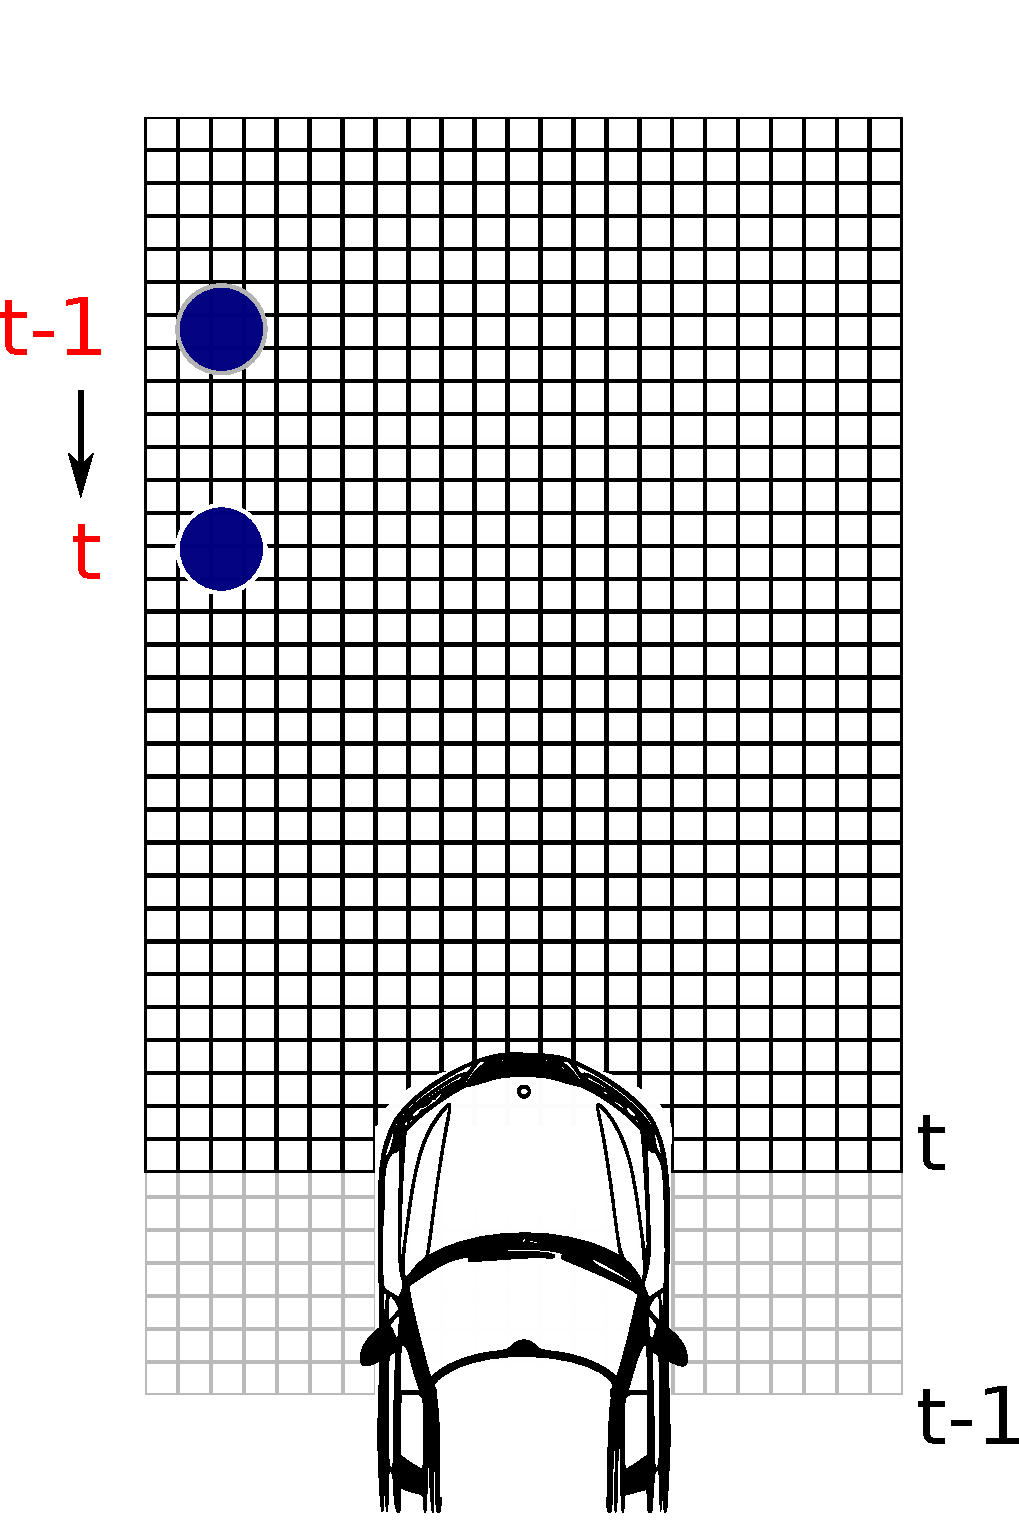
\includegraphics[scale=0.2]{img/fig:motion:algorithm:nonstatic:02}
		\end{figure}	
		  \end{column}
		  
		  \begin{column}{5cm}
			\begin{figure}[h]
			\center
			\includegraphics[scale=0.2]{img/fig:motion:algorithm:nonstatic:03}
		\end{figure}	
		  \end{column}
		 \end{columns}		 

	\end{frame}

	\begin{frame}
		\frametitle{Applying inverse of the Vehicle motion model}
		
		\begin{block}{Assumption}		
		Assume static environment constraints and apply the motion
		\end{block}		
		
		\begin{exampleblock}{Input}		
		Occupancy grid $+$ IMU data
		\end{exampleblock}

		\begin{alertblock}{Output}		
		Grid with correspondent cell mapping
		\end{alertblock}

		\begin{equation}
		\left[\begin{array}{c}x_t \\ y_t\\ \theta_t \end{array} \right] = 
		\left[\begin{array}{c} {\nu_t \over \omega_t} \sin(\omega_t \Delta t) \\ {\nu_t \over \omega_t} - {\nu_t \over \omega_t} \cos(\omega_t \Delta t) \\ \omega_t \Delta t \end{array}\right]
		\label{eq:circularmotion}
		\end{equation}
	\end{frame}	

	\begin{frame}
		\frametitle{Cell from different time steps, can be matched}

		  \begin{columns}[t]
		  \begin{column}{5cm}
			%\begin{alertblock}{Constraint}
			%	\begin{itemize}
			%	\item No overlap
			%	\item No merge
			%	\end{itemize}
			%\end{alertblock}
			\begin{equation}
			\ominus (P_{ij}) = \left[ \begin{array}{c} %P_{ji} \equiv 
			-x_{ij}\cos(\theta_{ij})-y_{ij}\sin(\theta_{ij}) \\
			x_{ij}\sin(\theta_{ij})-y_{ij}\cos(\theta_{ij}) \\
			-\theta_{ij} \end{array} \right] 
			\label{eq:invpose}
			\end{equation}
		  \end{column}
		  
		  \begin{column}{5cm}
			\begin{figure}[h]
			\center
			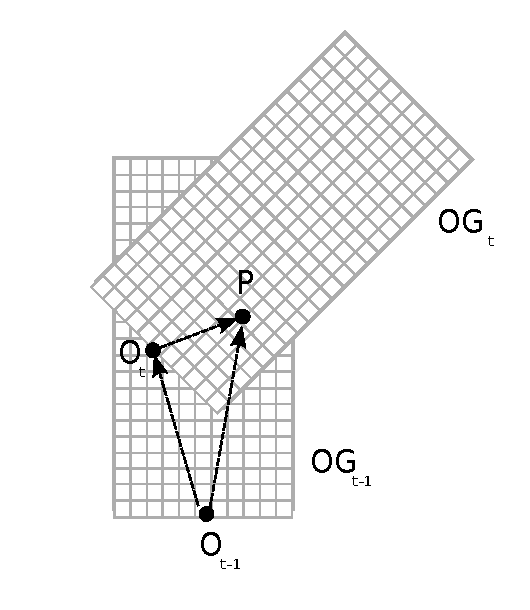
\includegraphics[scale=0.5]{../img/fig:translation}
			\end{figure}	
		  \end{column}
		 \end{columns}		 

	\end{frame}


\subsection{Phase 2}

	\begin{frame}
		\frametitle{Integrating new readings - Occupancy counter}		
		\begin{block}{Principle}
			Keep a counter of how many times a cell have been observed occupied, and how many times observed as free.
		\end{block}		
		
		  \begin{columns}[t]
		  \begin{column}{5cm}
		  \textbf{Initializing}
		  
		    \begin{equation}
			OC_t[i] =  \begin{cases} 1, & \mbox{ if $OG_t[i] > 0.5$} \\
			                       0, & \mbox{otherwise} \end{cases}
			\end{equation}

			\begin{equation}
			FC_t[i] = \begin{cases} 1, & \mbox{ if $OG_t[i] < 0.5$} \\
			                       0, & \mbox{otherwise} \end{cases}
			\end{equation}		  
		  
		  \end{column}
		  
		  \begin{column}{5cm}
		  \textbf{Updating}

			\begin{equation}
			OC_t[j] = OC_t[j] + OC_{t-1}[i]
			\end{equation}		  

			\begin{equation}
			FC_t[j] = FC_t[j] + FC_{t-1}[i]
			\end{equation}
		  
		  \end{column}
		 \end{columns}		 		
		
	\end{frame}

\subsection{Phase 3}

	\begin{frame}
		\frametitle{Classification in counter-based}
		
		\begin{block}{Definition}
		Classify in dynamic based on the ratio between OC and FC. 
		\end{block}		
		
		\begin{equation}
		MotionGrid_t[i] = \begin{cases} 1, & \mbox{$OG_t[i] > 0.5$ and} \\ & \mbox {$FC_t[i]>2\;  x \; OC_t[i]$} \\
		                                0, & \mbox{otherwise}\end{cases}
		\end{equation}		
		
	\end{frame}	

	\begin{frame}
		\frametitle{Solution summary}
		\begin{figure}[h]
			\center
			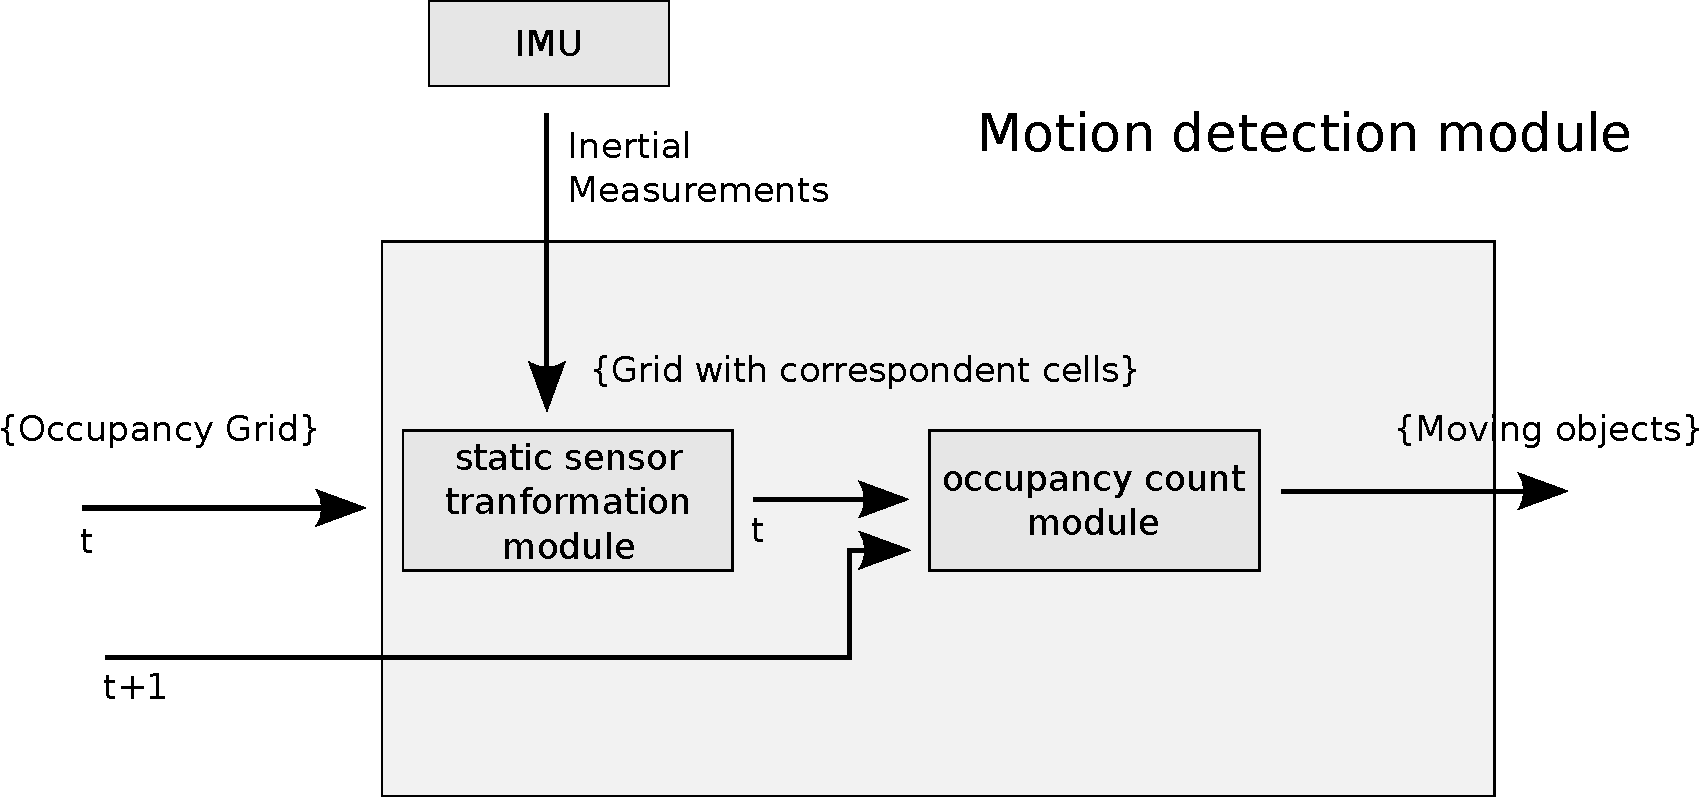
\includegraphics[scale=0.40]{../img/fig:motion:framework:motionmodule}
		 \end{figure}
		%\movie[width=3cm,height=2cm,poster]{la vidéo du FFFUUUU}{../videos/v8.mpeg}
	\end{frame}	

%%%%%%%%%%%%%%%%%%%%%%%%%%%%%

\section{Experiments}


\section{Results}

	\begin{frame}
		\frametitle{Use cases}
		3 use cases were chosen to assess our algorithm:
		\begin{itemize}
		\item Vehicles in urban area =  low speed + lot of rotation
		\item Vehicles in motorway = high speed + almost no rotation
		%\item Vehicle in roundabout
		\item Vehicle in static scenario = evaluate ground truth
		\end{itemize}						
	\end{frame}

	\begin{frame}
		\frametitle{Vehicles in urban area}
		
		\begin{columns}[t]
			\begin{column}[t]{5cm}
				\begin{figure}[h]
				\center
				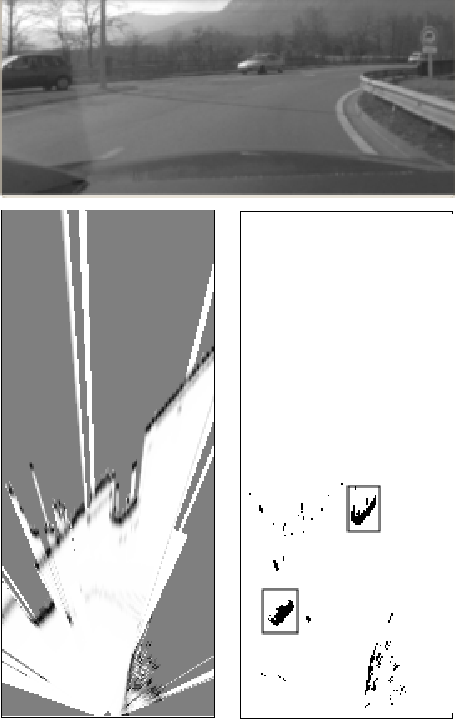
\includegraphics[scale=0.55]{../img/fig:result:scenetwocars}
				\end{figure}
			\end{column}
			\begin{column}[t]{5cm}
				\begin{exampleblock}{Positive}
				\begin{itemize}
				\item Visibility
				\end{itemize}
				\end{exampleblock}
				\begin{block}{Reason?}
				Bad rotation velocity data (IMU)
				\end{block}
			\end{column}
		\end{columns}		

	\end{frame}
	\begin{frame}
		\frametitle{Vehicles in motorway}
		\begin{columns}[t]
			\begin{column}[t]{5cm}
				\begin{figure}[h]
				\center
				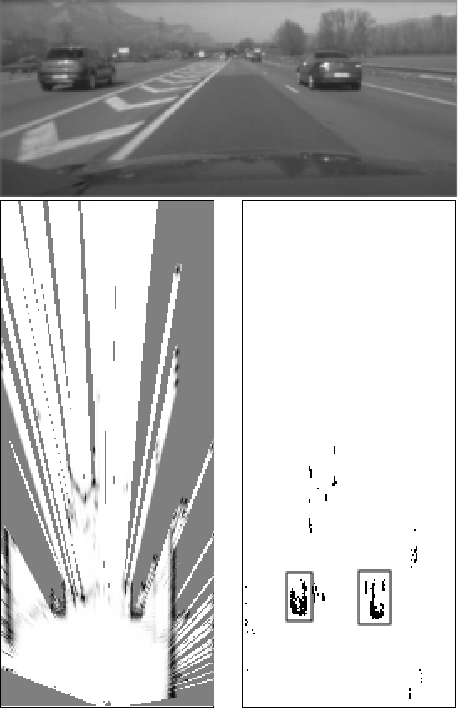
\includegraphics[scale=0.55]{../img/fig:result:scenetwocarshighway}
				\end{figure}
			\end{column}
			\begin{column}[t]{5cm}
				\begin{exampleblock}{Positive}
				\begin{itemize}
				\item Good results at high speed (when its most needed)
				\end{itemize}
				\end{exampleblock}
			\end{column}
		\end{columns}		

	\end{frame}

%	\begin{frame}
%		\frametitle{Vehicle in roundabout}
%		\begin{columns}[t]
%			\begin{column}[t]{5cm}
%				\begin{exampleblock}{Positive}
%				\begin{itemize}
%				\item Very dense pixels
%				\end{itemize}
%				\end{exampleblock}
%			\end{column}
%			\begin{column}[t]{5cm}
%				\begin{figure}[h]
%				\center
%				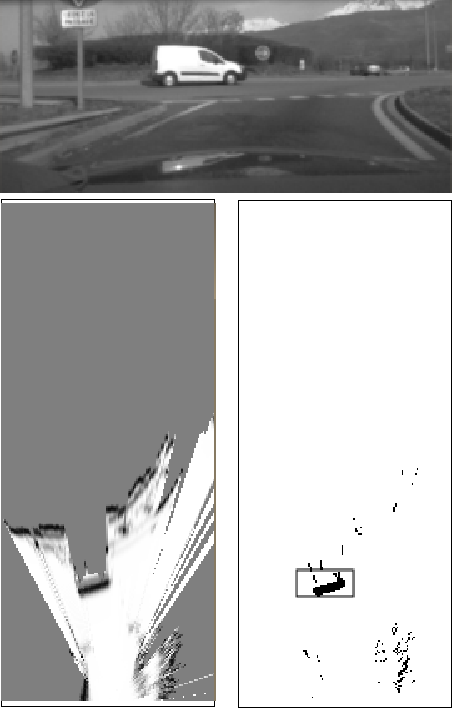
\includegraphics[scale=0.55]{../img/fig:result:scenetwocarrondepoint}
%				\end{figure}
%			\end{column}
%		\end{columns}
%	\end{frame}
	
	\begin{frame}
		\frametitle{Vehicle in static scenario}
		
		\begin{columns}[t]
			\begin{column}[t]{5cm}
				\begin{figure}[h]
				\center
				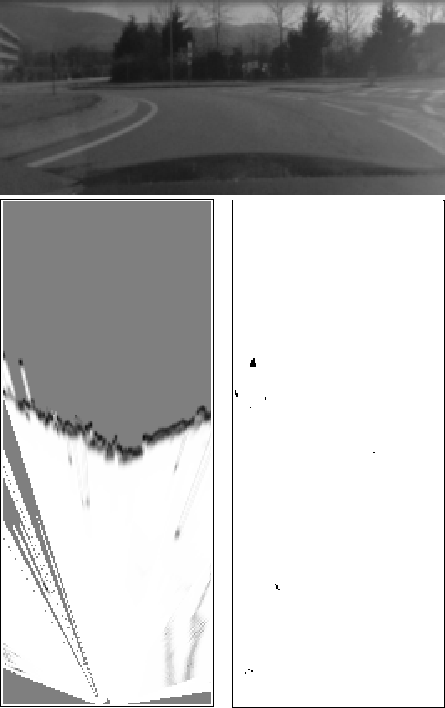
\includegraphics[scale=0.55]{../img/fig:result:scenestatic}
				\end{figure}
			\end{column}
			\begin{column}[t]{5cm}
				\begin{exampleblock}{Positive}
				\begin{itemize}
				\item Only few sparse pixels
				\item Easily removable with filters like:...
				\end{itemize}
				\end{exampleblock}		
			\end{column}
		\end{columns}
	\end{frame}			

	\begin{frame}
		\frametitle{Video}
		\centering
		$<$Show Video$>$
		
	\end{frame}		

	\begin{frame}
		\frametitle{Run time}

		\begin{alertblock}{Performance}
			Run in approximately 3.0ms in a 2.67Mhz processor
		\end{alertblock}		
		
		\begin{exampleblock}{Bright side}
			Still place for optimization
		\end{exampleblock}				
		
	\end{frame}	

\section{Conclusion}

	\begin{frame}
		\frametitle{Conclusion}
		
		\begin{block}{Benefits}
			\begin{itemize}
			\item easy to integrate with existing solutions
			\item faster way to classify
			\item still place for improvement
			\end{itemize}
		\end{block}		
		
		\begin{block}{Future work}
			\begin{itemize}
			\item Apply filters to reduce the noise
			\item Fuse with other sensors to reduce the IMU data precision dependency
			\end{itemize}
		\end{block}
		
	\end{frame}

	\begin{frame}{That is it..}
	\begin{alertblock}{}
		\centering
		Questions?
	\end{alertblock}
	\end{frame} 	
 	
\bibliographystyle{apalike}%abbrvnat%alpha
\bibliography{../report}{} 	

\end{document}